\chapter{Project 3: Pig Game}

\section{Overview}
This project adds on to the lessons from the last project. In addition to our single LED and button,
we'll now have a more complex seven-segment display and a second button to work with.
Over the course of this project, you will:
\begin{itemize}
    \item Expand the circuits from previous projects with more components
    \item Wire up a complex component that requires many input wires
    \item Write a program that will play a simple two-player game using the components
\end{itemize}
At the end of this project, your microcontroller should run a MicroPython program that allows
two players to take turns rolling a die. The first player to reach 100 points wins the game.
\begin{figure}[H]
\centering
    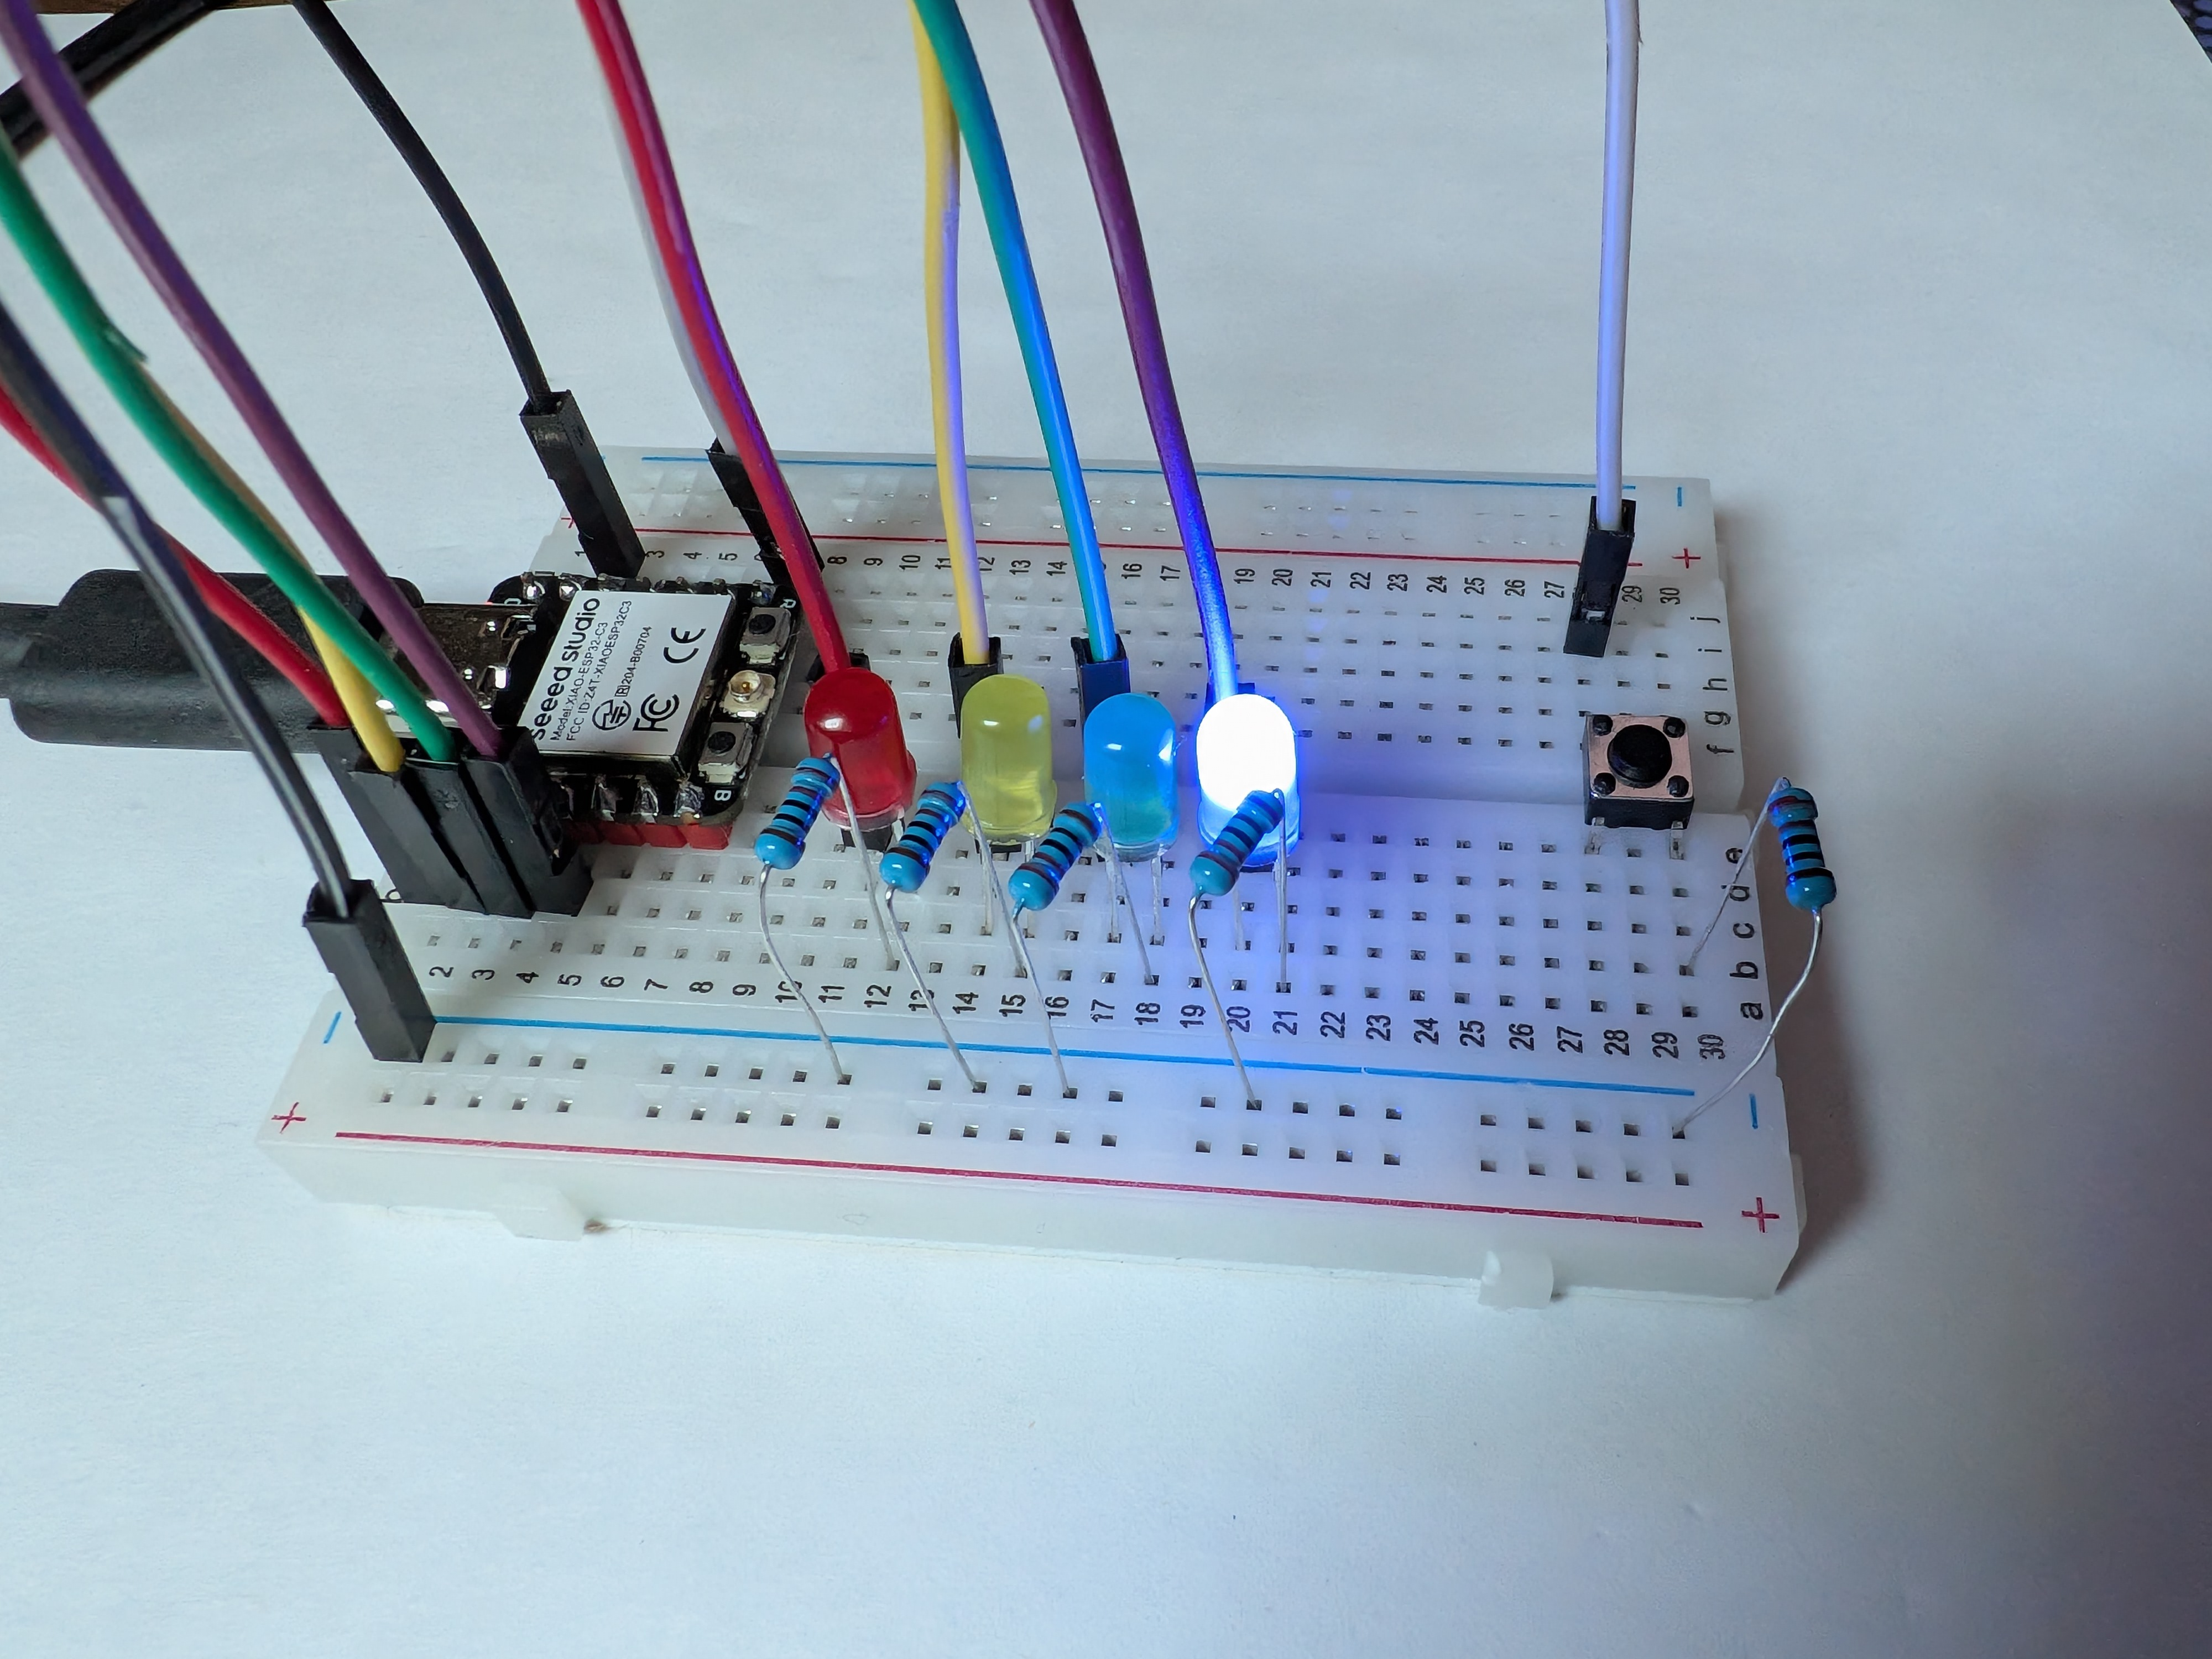
\includegraphics[width=.6\linewidth]{project_3/success!.jpg}
    \caption{The end result should look something like this}
\end{figure}

\pagebreak

\section{Directions}

\subsubsection{Remove previous components}
Before beginning, remove any components from prior chapters including LEDs, buttons, and wires. You may leave the
microcontroller attached to the breadboard.

\subsection{Creating the circuit}
Using jumper cables, you will be assembling a circuit between your microcontroller, your breadboard,
some LEDs, a pushbutton, and a 220\si{\ohm} resistor for the display.

\subsubsection{Attach the microcontroller to the breadboard}
Carefully insert the pins at the bottom of your microcontroller into the breadboard, making sure that the microcontroller is oriented such that:
\begin{itemize}
    \item The pin labeled \textbf{5V} is inserted in hole at \textbf{Column H, Row 1} of the breadboard (or \textbf{H1}, for short)
    \item The pin labeled \textbf{GPIO2} is inserted in hole \textbf{D1} of the breadboard
    \item The pin labeled \textbf{GPIO20} is inserted in hole \textbf{H7} of the breadboard
    \item the pin labeled \textbf{GPIO21} is inserted in hole \textbf{D7} of the breadboard
\end{itemize}
You may need to apply more pressure than expected to seat the microcontroller properly in the breadboard. When its over, it should look like this:

\begin{figure}[H]
    \centering
    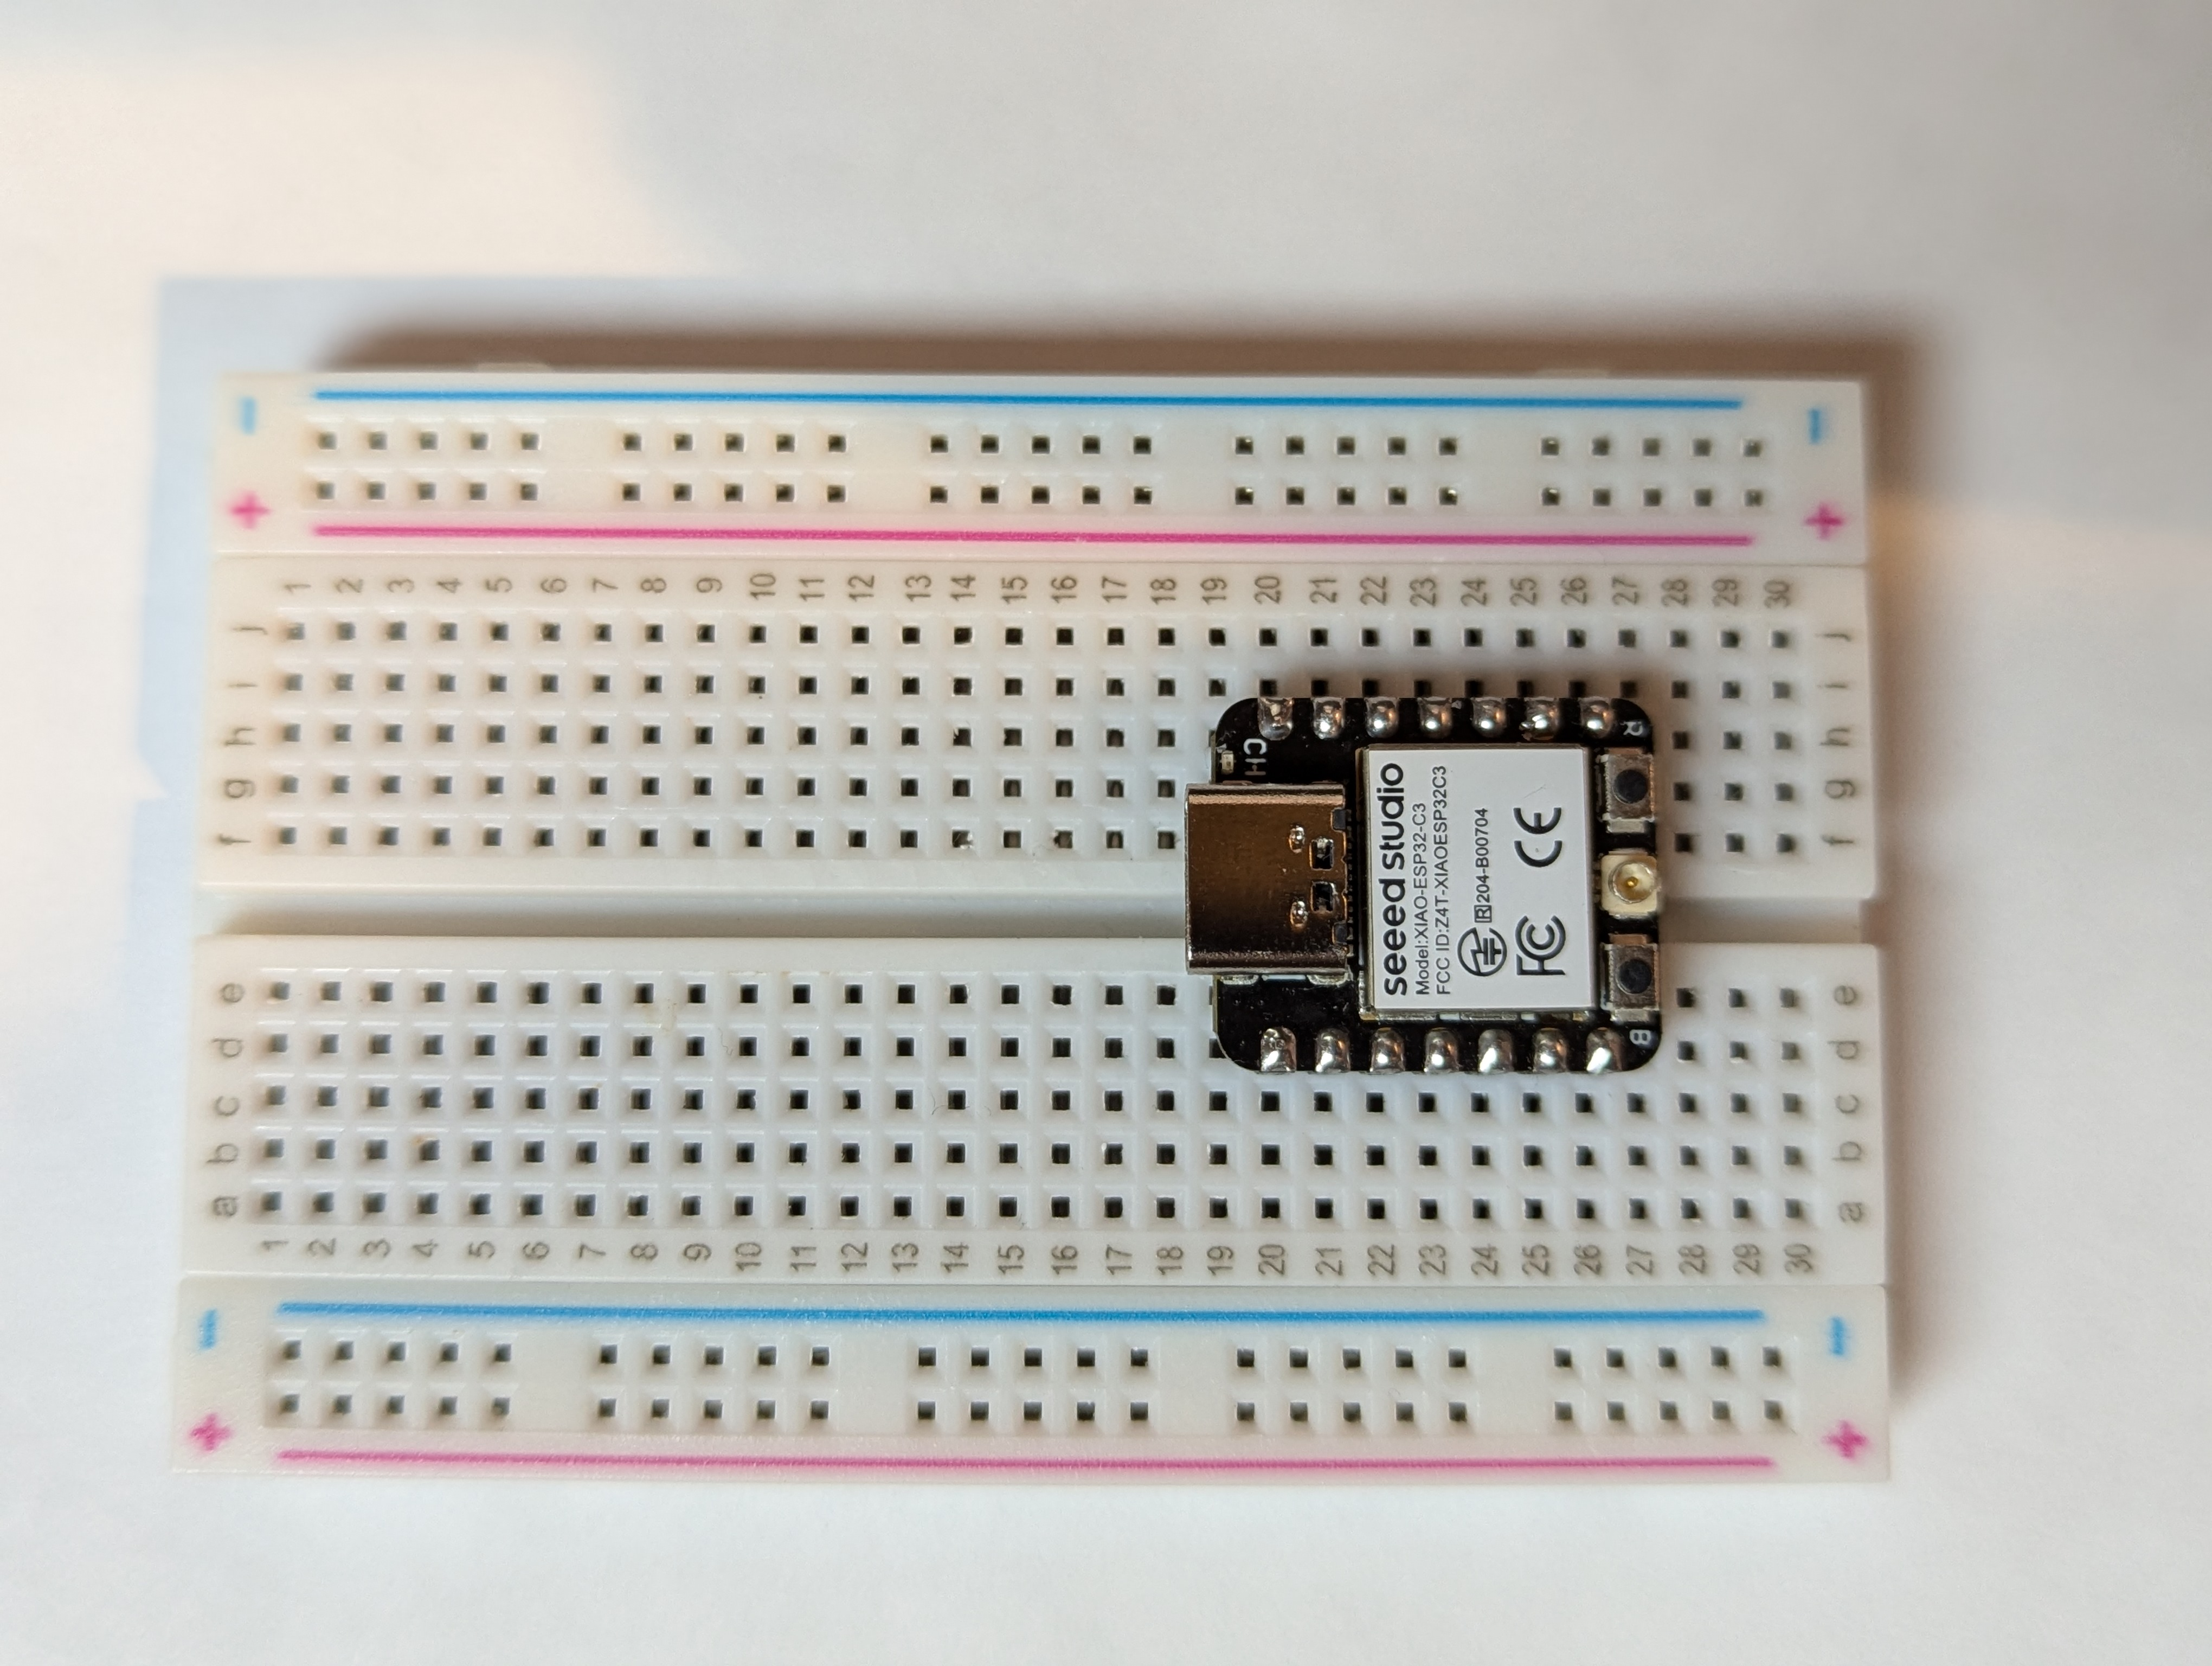
\includegraphics[width=.6\linewidth]{common/microcontroller_seated_in_breadboard.jpg}
    \caption{So far, so good!}
\end{figure}

\subsubsection{Connect the Display, Buttons, and Resistor}
\begin{itemize}
    \item Place the seven-segment display in the board with the top left pin in \textbf{G13}, the top right pin
    in \textbf{G17}, the bottom left pin in \textbf{C13}, and the bottom right pin in \textbf{C17}.
    \item Place a button button so that one connected set of pins (refer to \ref{button_basics} for an example) is in \textbf{E24}
    and \textbf{F24} and the other set is in \textbf{E26} and \textbf{F26}.
    \item Place a second button so that one connected set of pins is in \textbf{E28} and \textbf{F28}
    and the other set is in \textbf{E30} and \textbf{F30}.
    \item Finally place a resistor between \textbf{I15} and the top negative rail.
\end{itemize}

You should be left with something that looks like this:
\begin{figure}[H]
    \centering
    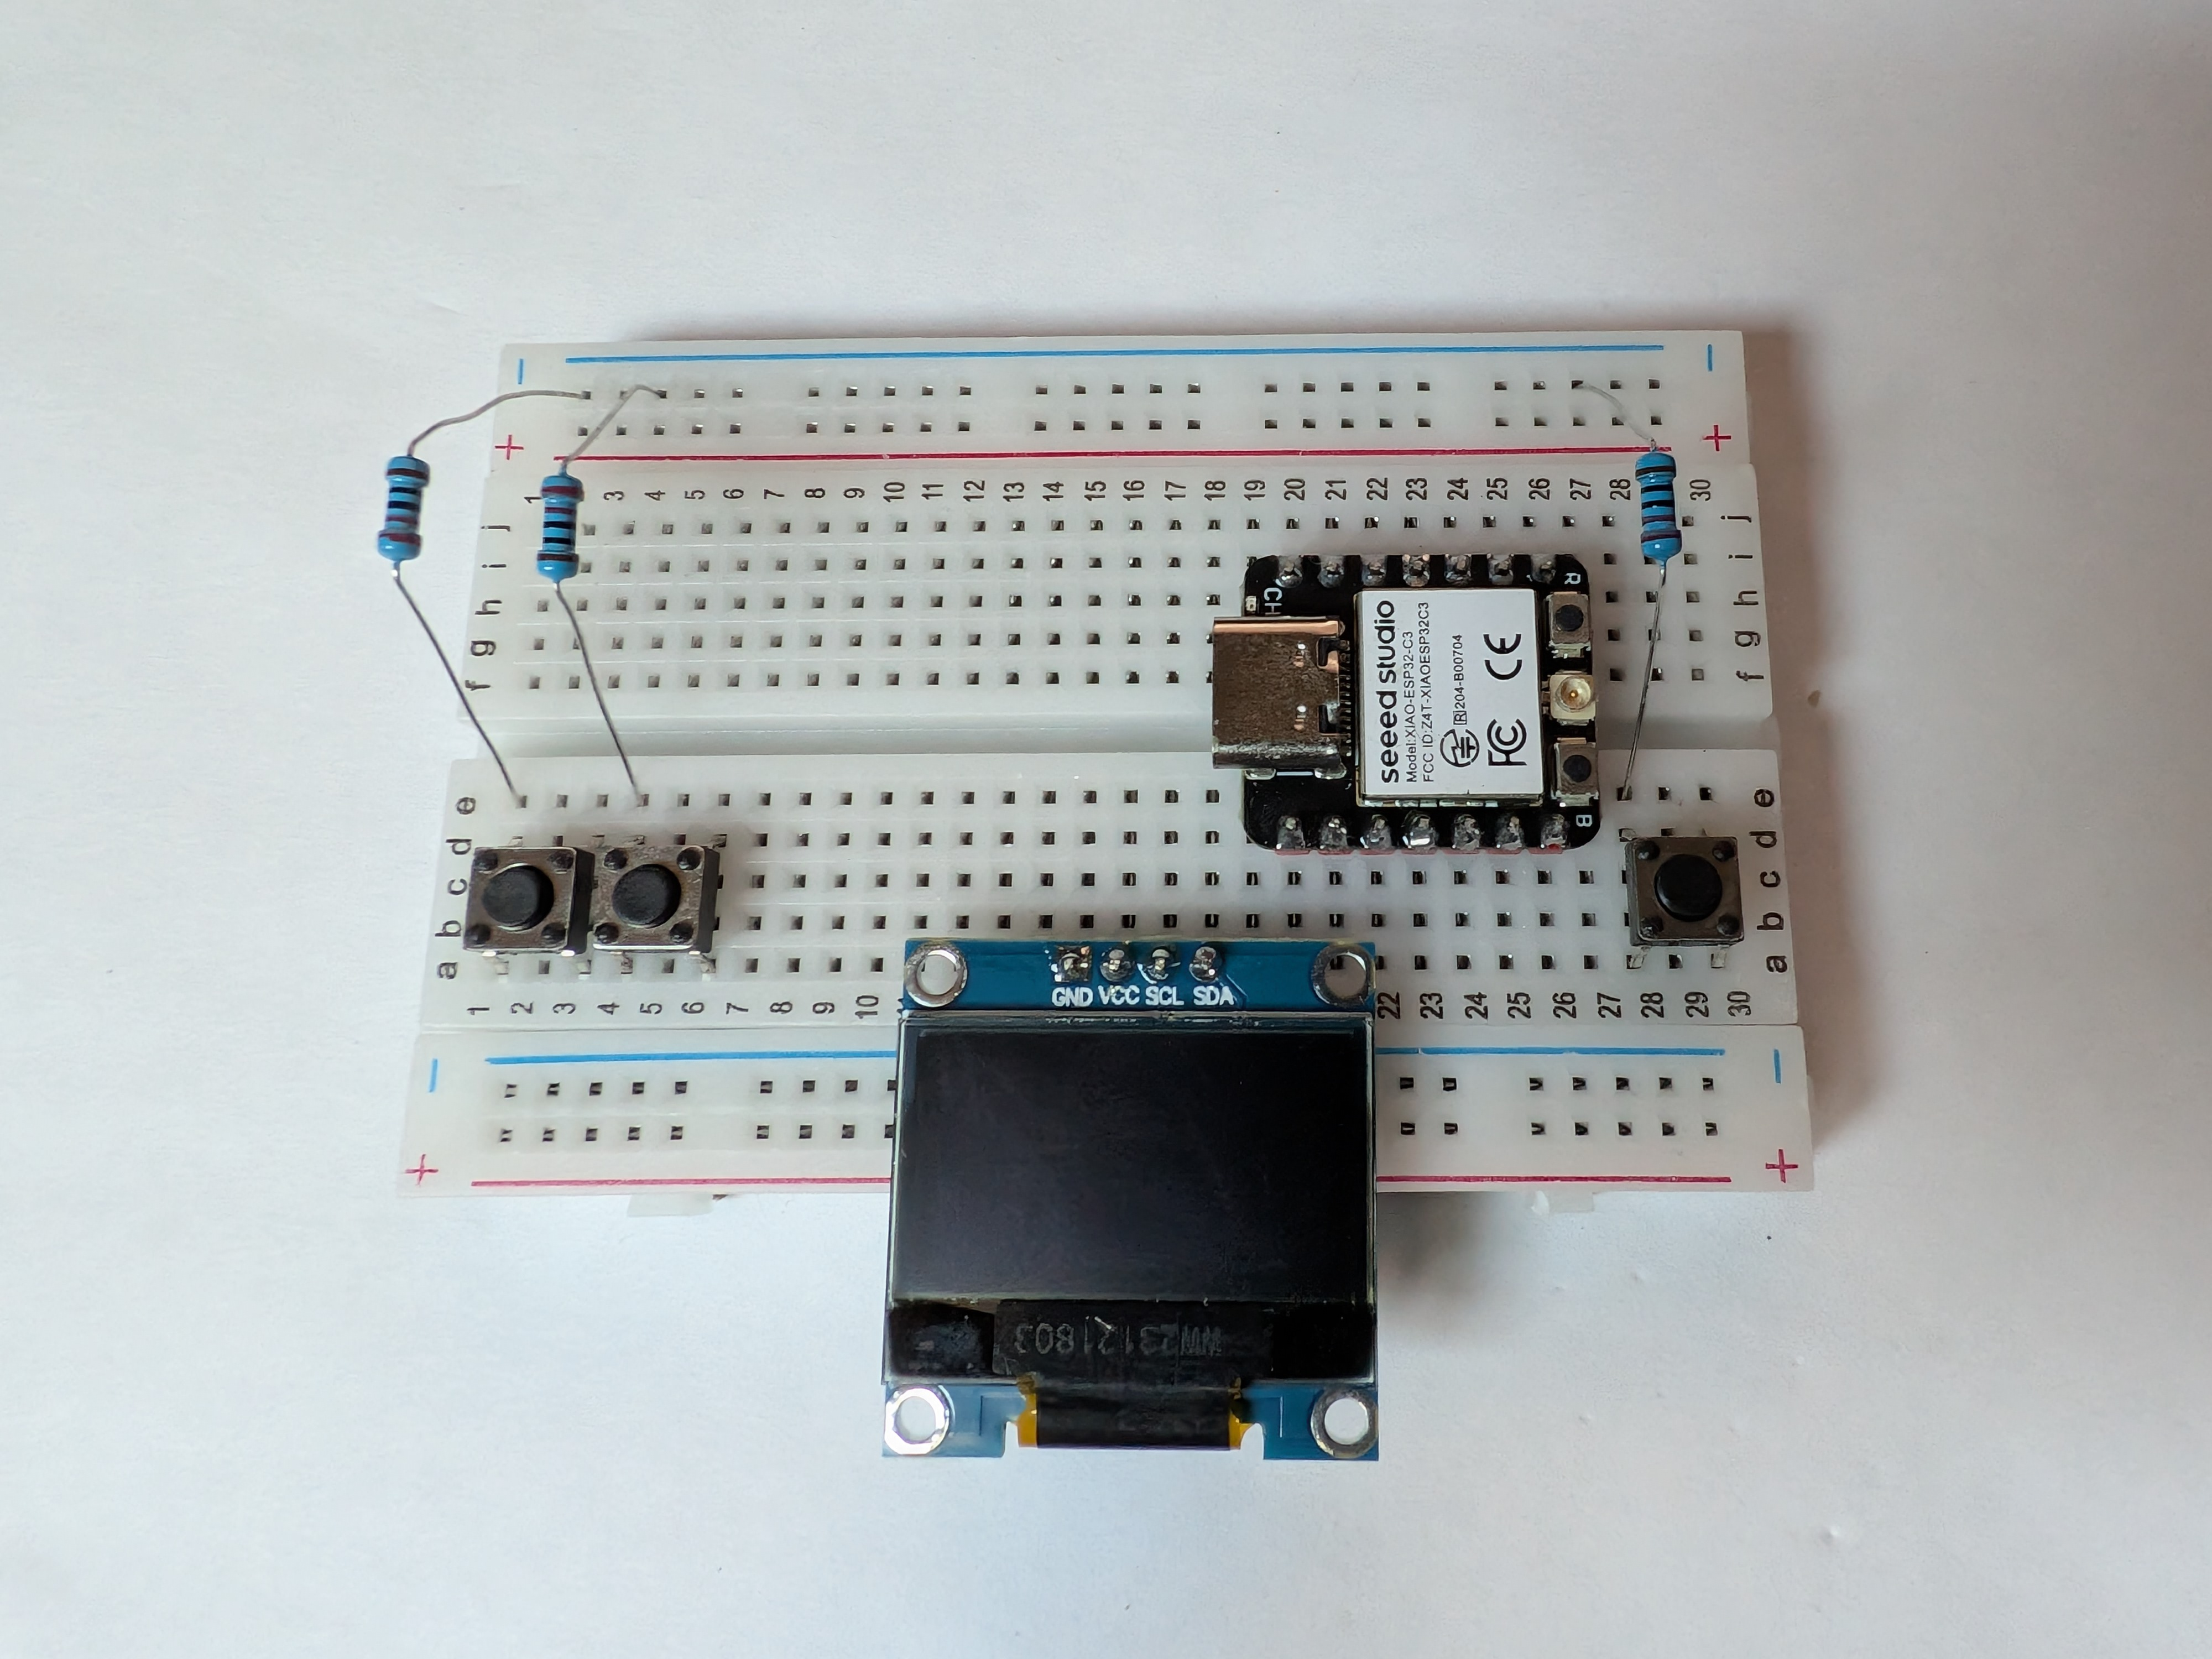
\includegraphics[width=.55\linewidth]{project_3/components_placed.jpg}
    \caption{All of the components except for the jumper wires are now placed.}
\end{figure}

\subsubsection{Connect the necessary jumper wires}
\begin{itemize}
    \item Place one end of a black jumper wire into hole \textbf{J2} of the breadboard and the other end into
    the top negative rail (the blue one). This will provide a ground path for all of the components.
    \item Place a yellow jumper wire between \textbf{J4} and \textbf{J13}.
    \item Place a green jumper wire between \textbf{J5} and \textbf{J14}.
    \item Place a blue jumper wire between \textbf{J6} and \textbf{J16}.
    \item Place a purple jumper wire between \textbf{B6} and \textbf{J17}.
    \item Place a yellow jumper wire between \textbf{B5} and \textbf{A16}.
    \item Place a green jumper wire between \textbf{B4} and \textbf{A14}.
    \item Place a purple jumper wire between \textbf{B3} and \textbf{A13}.
    \item Place a white jumper wire between \textbf{B2} and \textbf{J30}.
    \item Place a white jumper wire between \textbf{B1} and \textbf{J26}.
    \item Place a black jumper wire between \textbf{J24} and the top negative rail.
    \item Place a black jumper wire between \textbf{J28} and the top negative rail.
\end{itemize}

You should be left with something that looks like this:
\begin{figure}[H]
    \centering
    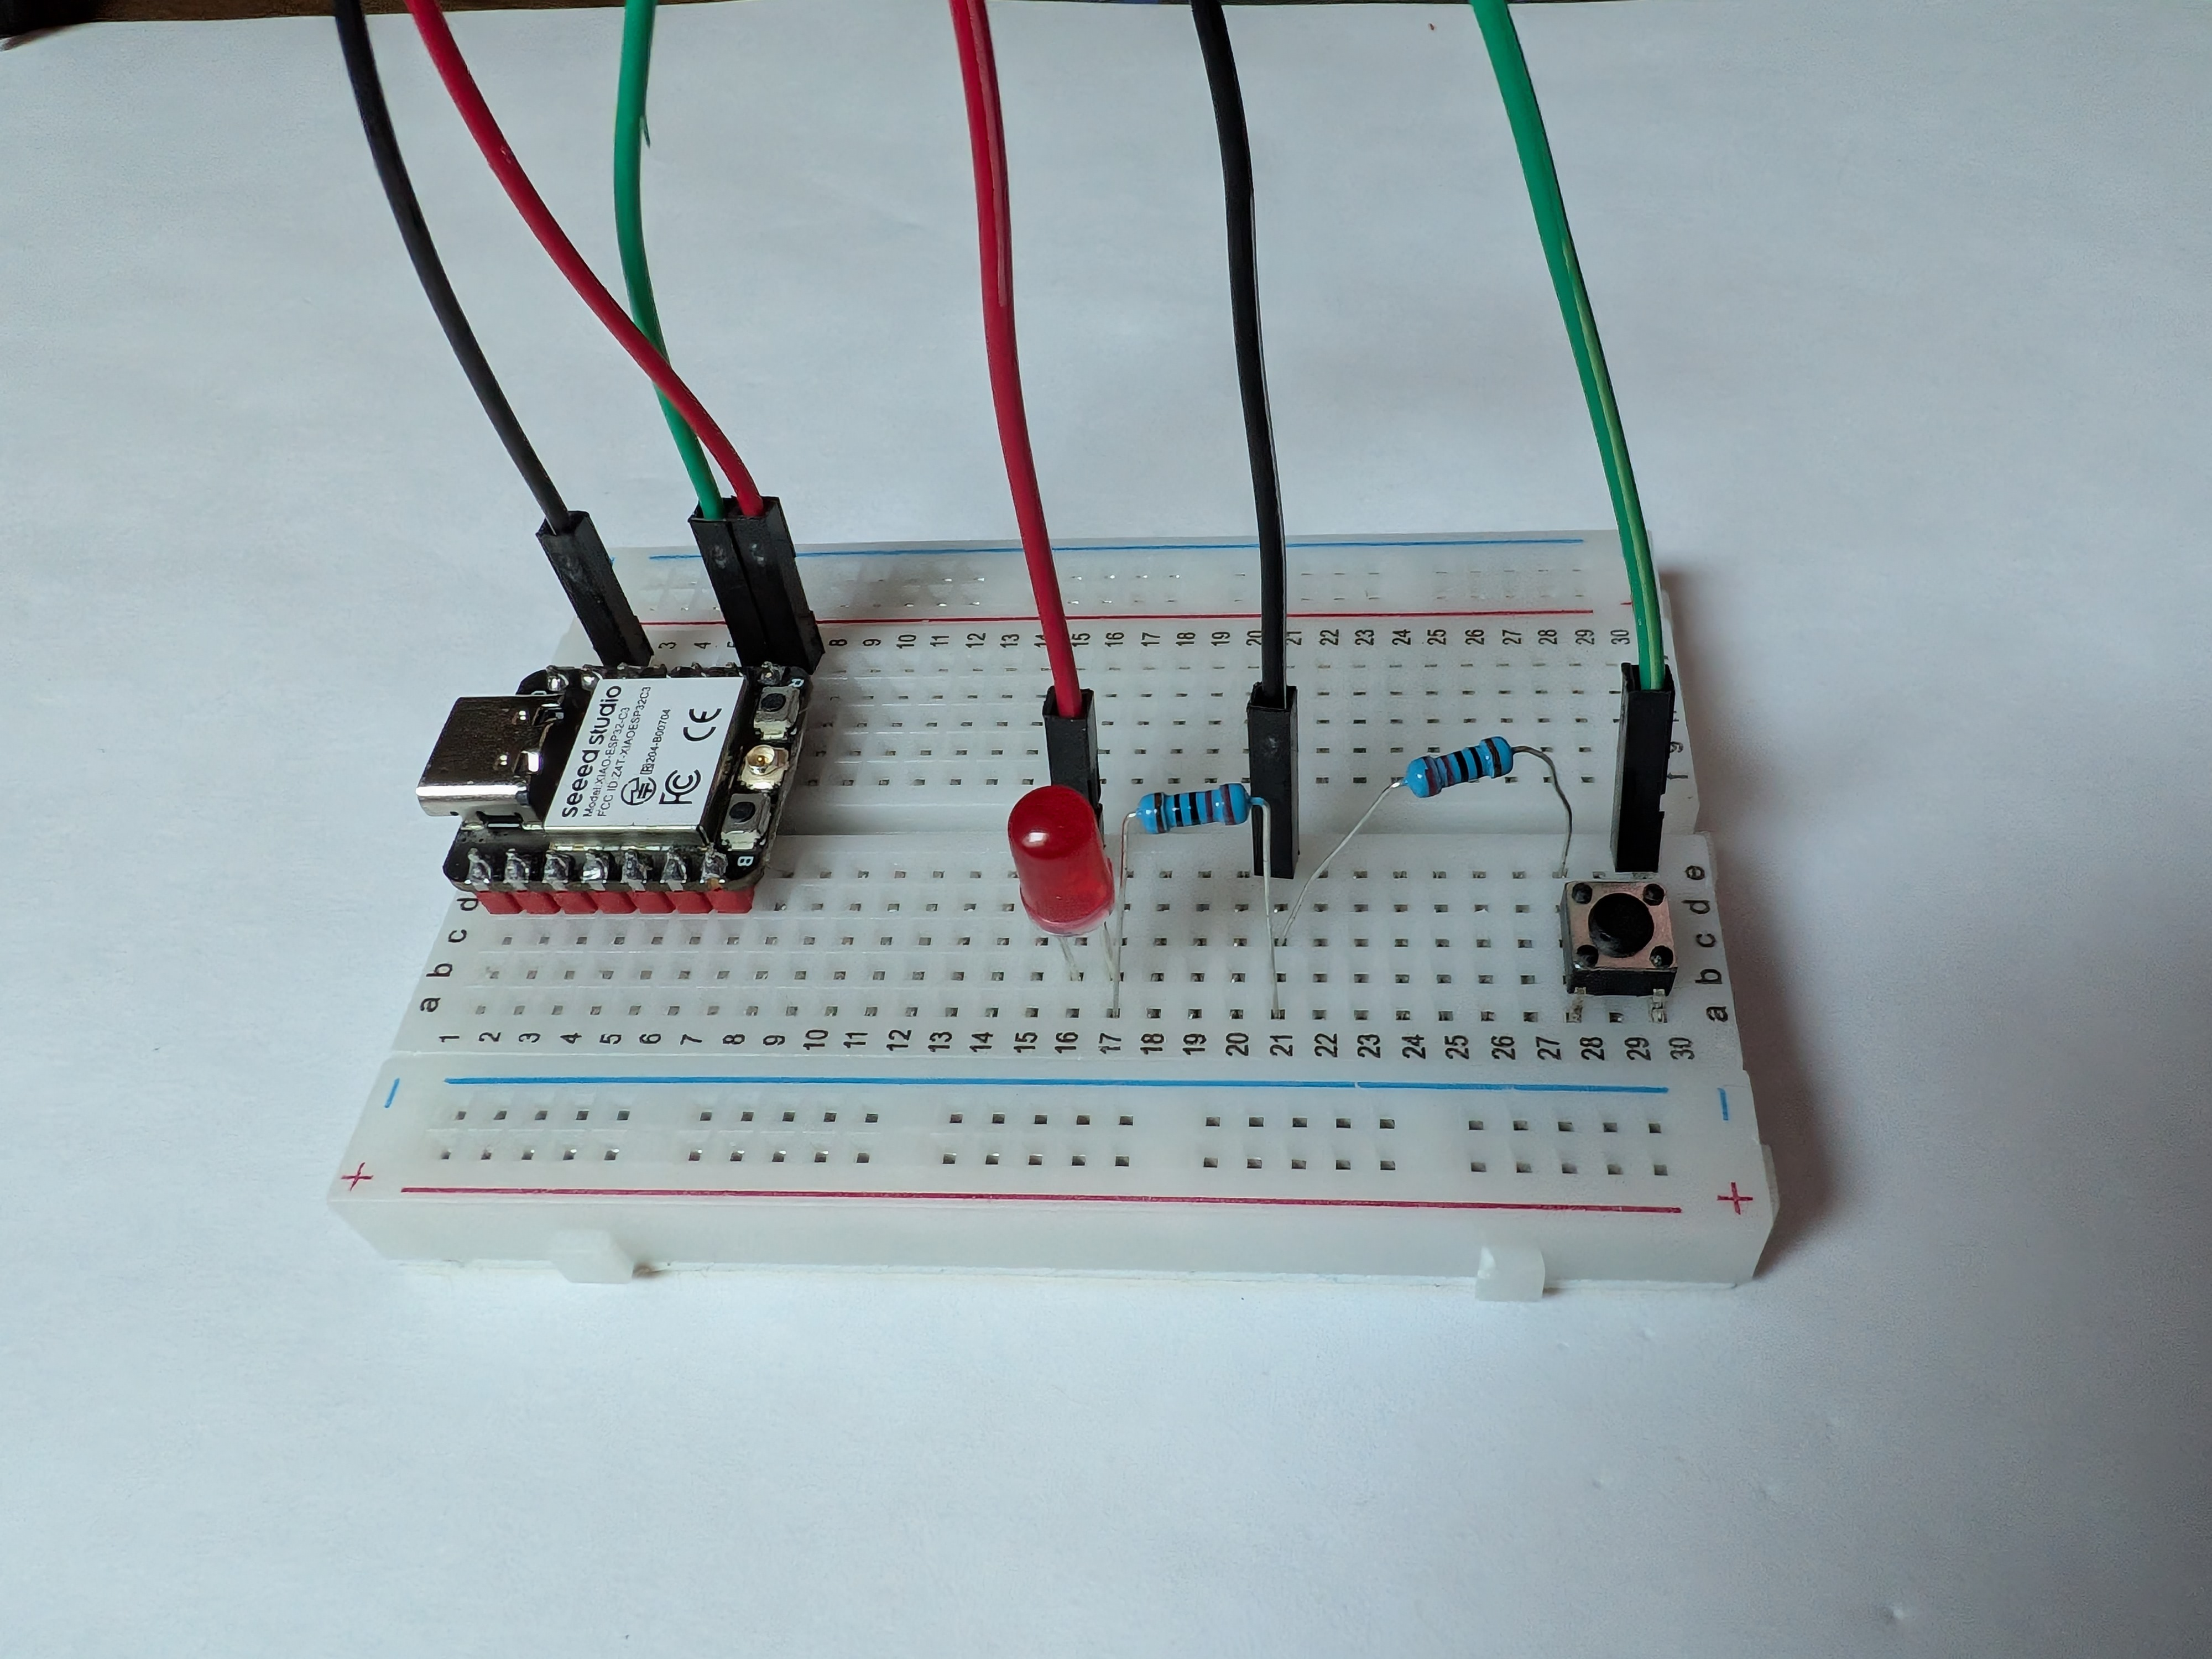
\includegraphics[width=.55\linewidth]{project_3/all_wired_up.jpg}
    \caption{All components and wires are now installed}
\end{figure}

\subsection{Programming the microcontroller}

Once all of the wiring is correct, connect the USB cable to the microcontroller and load the IDE to
access it. Refer back to Chapter \ref{ide} for instructions.

Click on the file named "project\_3\_pig\_game.py". This will load the code in the editor for this section.
Read through the comments and the code to get a sense for how it works. Once you are ready, you can
click the blue play button in the upper left of the window to start the game.

The game will start with player 1 rolling the die using the right-most button. As long as the player does not
roll a 1, they can continue to accumulate points. If they roll a 1, they lose all of their points accumulated
during that turn and the next player gets a turn. If they roll any other number, they can choose to end their
turn and save the points by pressing the left button. Play continues to pass back and forth until one player
reaches the win limit of 100 saved points and wins the game.

\section{Review}
In this project, we learned how we can add interactivity to a circuit by using momentary pushbuttons.
These buttons can be read from the microcontroller's code to run a piece of code (called an interrupt)
whenever they are pressed.

\section{Possible Extensions}
If you want to do some experimentation, try these:

\begin{itemize}
    \item Add an indicator to show on the board which player's turn it is. You might add some LEDs from the kit, or maybe use the decimal point on the seven-segment display.
    \item Try changing the code to implement one or more of the variations on the Pig game: \url{https://en.wikipedia.org/wiki/Pig_(dice_game)#Variations}
\end{itemize}
